\section{From Stability to Effectiveness: Overcoming Lazy Optimization}
\label{sec:trade-off-rl}
\begin{figure}[t!]
  \centering
  \begin{minipage}[t]{0.49\linewidth}
    \centering
    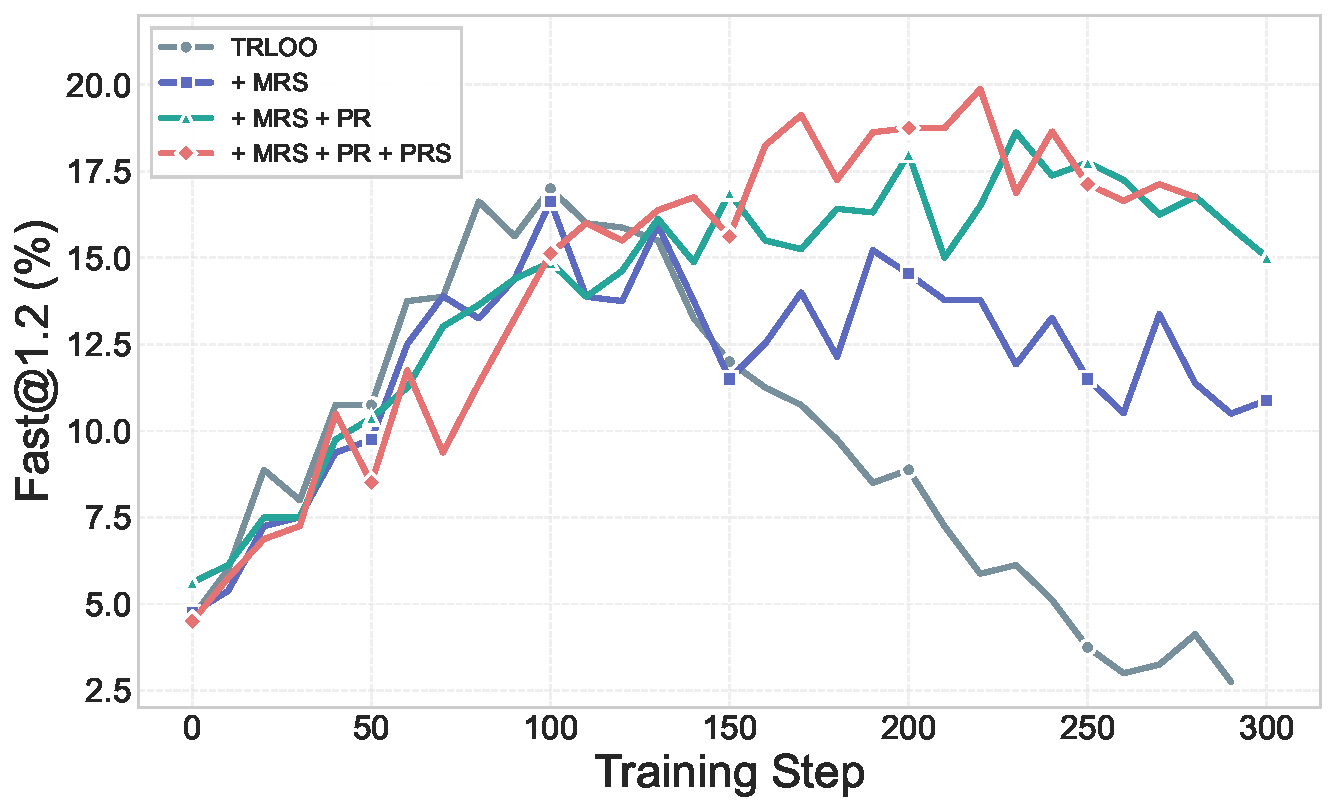
\includegraphics[width=\linewidth]{figures/fast12_comparison.pdf}
  \end{minipage}\hfill
  \begin{minipage}[t]{0.49\linewidth}
    \centering
    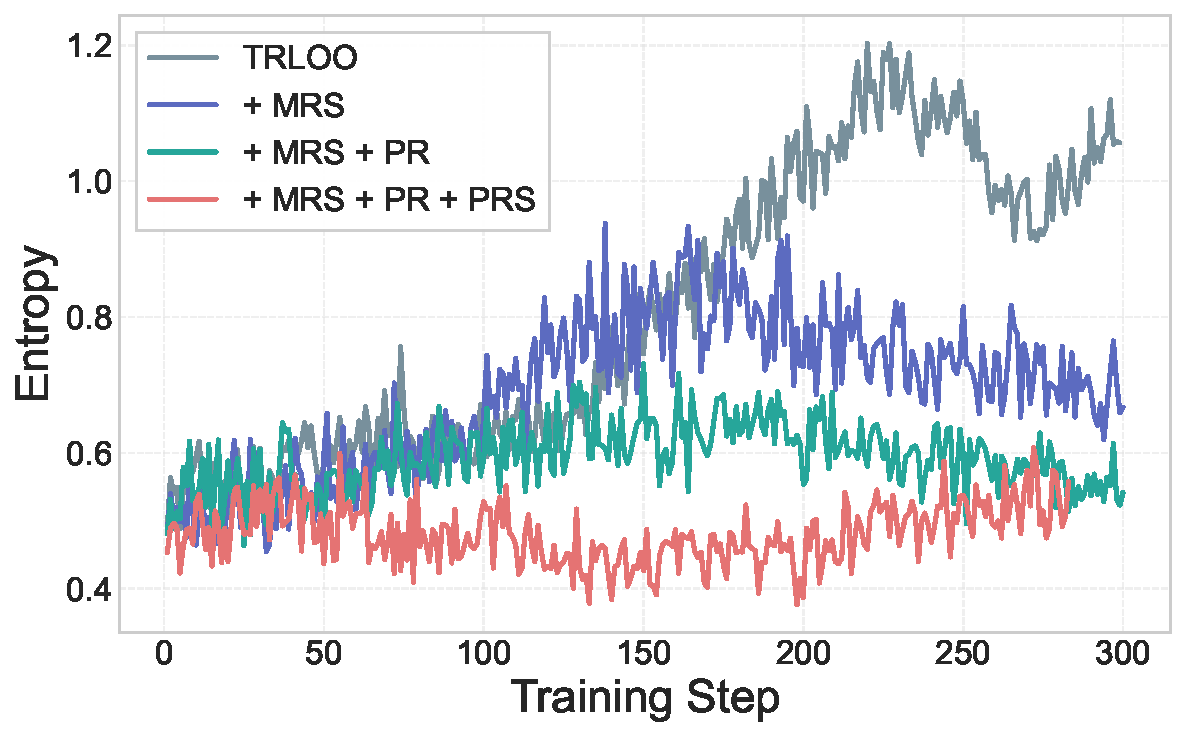
\includegraphics[width=\linewidth]{figures/entropy.pdf}
  \end{minipage}
  \caption{\textbf{Left}: Fast@1.2 at turn~3 over training steps. While MRS stabilizes training, profiling-based methods (PR and PRS) are required to significantly improve the stricter Fast@1.2 metric. \textbf{Right}: Entropy over training steps. While MRS improves training stability, PR and PRS further enhance stability on top of MRS. Additional training dynamics are shown in Figure~\ref{fig:training-dynamics}.}
  \label{fig:tradeoff}
\end{figure}
With \env{} and TRLOO, long-term RL training becomes feasible, yet the ``lazy optimization'' issue persists as discussed in \S\ref{sec:pitfalls} and Figure~\ref{fig:pitfalls}. We systematically investigate this bottleneck through two hypotheses. Hypothesis~1: the saturation is caused by optimization instability arising from training--inference mismatch. Hypothesis~2: the optimization objective remains misaligned with \emph{meaningful} speedup, incentivizing low-impact solutions.

\subsection{Hypothesis 1: Training Instability}
Our initial speculation was that this premature saturation stemmed from training instability. Training--inference mismatch~\citep{yao2025offpolicy,liu-li-2025-rl-collapse} is a fundamental challenge in RL for LLMs, where discrepancies between the rollout (inference) and training engines induce off-policy drift. Theoretically, this drift can lead to gradient variance and reward collapse, preventing the model from reaching higher performance peaks.

To investigate this, we monitor training dynamics via entropy, gradient norms, and perplexity (Figure~\ref{fig:training-dynamics}). As observed, the multi-turn RL for kernel generation run exhibits excessively high values across these metrics, clearly indicating training instability. Following \citet{liu-li-2025-rl-collapse}, we adopt geometric Mismatch Rejection Sampling (MRS) to mitigate this drift. We compute the geometric-mean importance ratio
\begin{equation}
    w=\exp\!\Big(\tfrac{1}{|T|}\sum_{t\in T}\log\frac{\pi_{\text{train}}(a_t\mid s_t)}{\pi_{\text{rollout}}(a_t\mid s_t)}\Big),
\end{equation}
retaining samples only if $w\in[0.999,1.001]$. Additionally, we enforce a strict token-level veto: the entire sequence is rejected if the likelihood ratio $\pi_{\text{train}}/\pi_{\text{rollout}}$ for any single token drops below $10^{-4}$.

As visualized in Figure~\ref{fig:training-dynamics}, MRS successfully stabilizes the training dynamics. However, Figure~\ref{fig:tradeoff} reveals a critical insight: while mismatch correction prevents early collapse (smoothing the learning curve), it does not fundamentally lift the performance ceiling of Fast@1.2. This indicates that while Hypothesis 1 effectively accounts for the training instability, addressing it alone does not fully resolve the performance saturation. Consequently, this directs our focus to the optimization objective itself.

\subsection{Hypothesis 2: Misaligned Objective}
Given that improving stability alone is insufficient, we speculate that the standard reward signal fails to distinguish between trivial improvements and meaningful bottlenecks. While a kernel may be correct and achieve some speedup, it might still fail to address the true performance bottlenecks. To move from producing merely \emph{correct} kernels to \emph{effective} ones, we must make rewards \emph{bottleneck-aware}.

\paragraph{Profiling-based Rewards (PR)}
\wl{Modified} A key symptom of this misalignment is the tendency for models to optimize trivial sub-operations (e.g., replacing a simple summation operation) without affecting the dominant bottlenecks in the computation. As demonstrated in the case study of lazy optimization versus better fusion (Figure~\ref{fig:profiling-lazy-optim}), in the lazy optimization case, the model-generated kernel accounted for only $0.014\%$ of the total CUDA execution time, indicating that the kernel optimization did not affect the main bottlenecks. In contrast, with better fusion, the model generated kernels that covered $86.15\%$ of the total CUDA runtime, resulting in better and more meaningful speedup.

To formalize this intuition, we leverage the profiling toolkit in \env{} to isolate the runtime contribution of the generated kernels ($T_{\text{generated}}$) from the overall CUDA execution time ($T_{\text{total}}$). We define the profiling ratio as:
\begin{equation}
\operatorname{PR}_{i,t} \;=\; \frac{T_{\text{generated}}}{T_{\text{total}}}.
\end{equation}
Intuitively, $\operatorname{PR}_{i,t}$ assigns higher credit when the candidate optimizes kernels that dominate the end-to-end runtime. We then augment the per-turn reward with this signal (applied only to correct kernels):
\begin{equation} 
\label{eq:pr}
R_{i,t} = C(y_{i,t}) + C(y_{i,t})\cdot \operatorname{speedup}_{i,t} + C(y_{i,t})\cdot \operatorname{PR}_{i,t}.
\end{equation}
This encourages the model to focus on kernel optimizations that contribute significantly to performance, explicitly driving learning toward optimizations with larger real speedup. Besides, since $PR_{i,t}$ is bounded in $[0,1]$, the $\operatorname{speedup}$ term naturally dominates, preventing the model from maximizing coverage via inefficient code.
% Although maximizing $T_{generated}$ alone could encourage slow kernels, the coupled $\operatorname{speedup}$ term in Eq. (8) strictly penalizes regression, forcing the model to seek high coverage without sacrificing efficiency.

\paragraph{Profiling-based Rejection Sampling (PRS)}
Even with bottleneck-aware rewards, the exploration process can still be dominated by a high volume of low-impact (``lazy'') samples. To further filter the training distribution, we introduce \emph{profiling-based rejection sampling} (PRS). For each sample $(i,t)$, we retain it with probability:
\begin{equation}
p_{i,t}
=\mathrm{clip}\!\left(\frac{\operatorname{PR}_{i,t}-\tau}{s},\,0,\,1\right),
\label{eq:prs}
\end{equation}
where $\tau$ is a cutoff threshold and $s$ controls the softness of the filter. In our experiments, we fix $\tau=0.3$ and $s=0.1$. We ablate the design choice of PRS in Appendix~\ref{ap:prs-ablations}.\wl{Modified}

\subsection{Empirical results}
Figure~\ref{fig:tradeoff} confirms this staged diagnosis. MRS improves training stability but does not, by itself, raise the Fast@1.2 ceiling. Furthermore, adding PR and PRS substantially lifts Fast@1.2. And the stability is even further improved by PR and PRS as shown in Figure~\ref{fig:tradeoff} (Right) and Figure~\ref{fig:training-dynamics}.